% File: approx.tex
% Date: Mon Jul 08 21:39:23 2013 +0800
% Author: Yuxin Wu <ppwwyyxxc@gmail.com>

\section{Approximation}
Note that $ e^{-1} = \sum_{i=0}^{\infty}\dfrac{(-1)^i}{i!}$,
which indicates that $\Pr{X=k}\approx \dfrac{e^{-1}}{k!},D_n \approx e^{-1}n! $. Now we focus on this two approximations.

\subsection{Approximation of $ \Pr{X=k}$}
Let $ Y$ be a random variable such that $ Y\sim \text{Poisson}(1)$, then
we have $ \Pr{Y=k} = \dfrac{1}{ek!}$.
Therefore when $ n$ is large enough,
$ X$ approximately obeys \emph{Poisson distribution} with the parameter $ 1$.

Actually, even when $ n$ is small,
there is very little difference between $ \Pr{X=k}$ and $ \Pr{Y=k}=\dfrac{1}{ek!}$,
as shown in \figref{diff}.

\begin{figure}[H]
  \centering
  \subfigure[$n$=3]{
    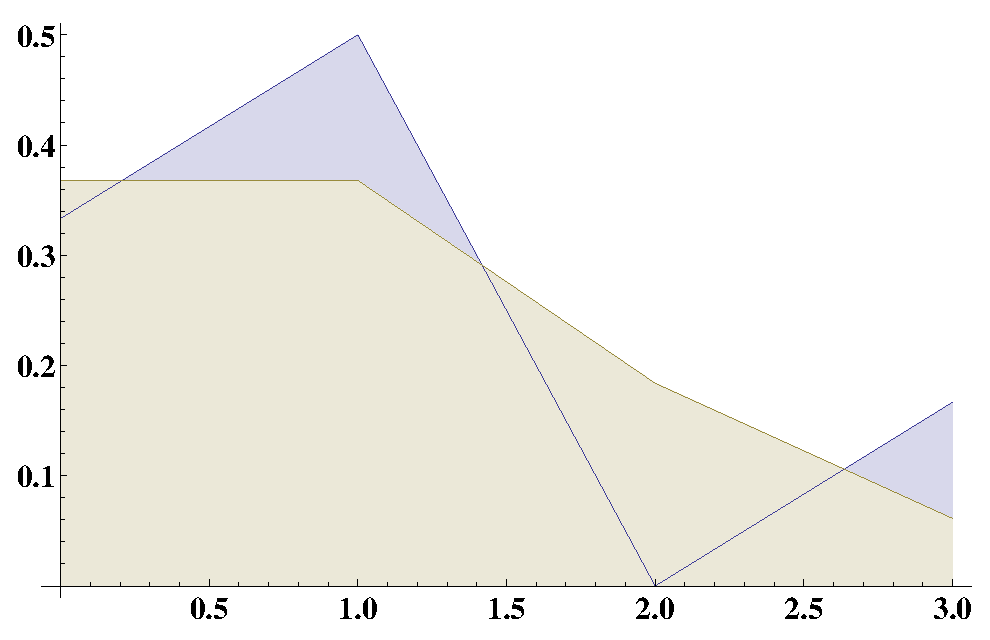
\includegraphics[scale=0.4]{img/n3.eps}
  }
  \subfigure[$ n$=4]{
    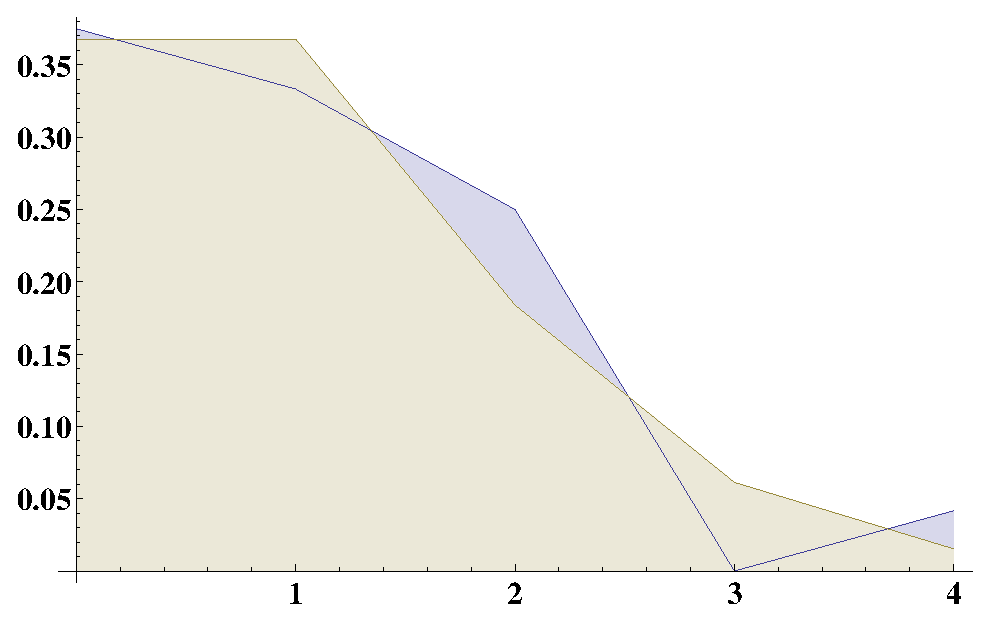
\includegraphics[scale=0.4]{img/n4.eps}
  }
  \subfigure[$n$=5]{
  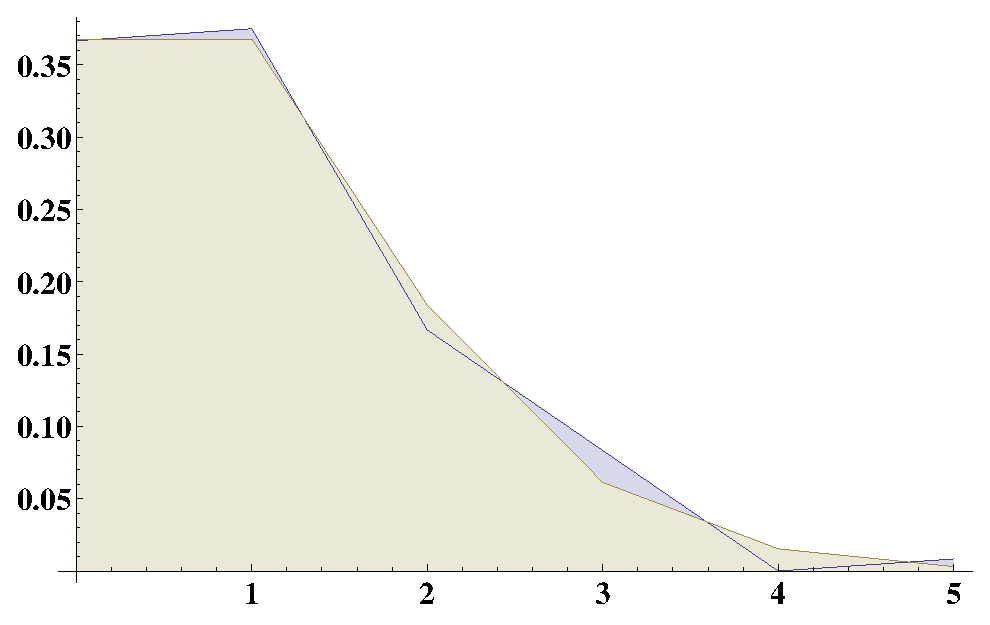
\includegraphics[scale=0.4]{img/n5.eps}
  }
  \subfigure[$ n$=6]{
  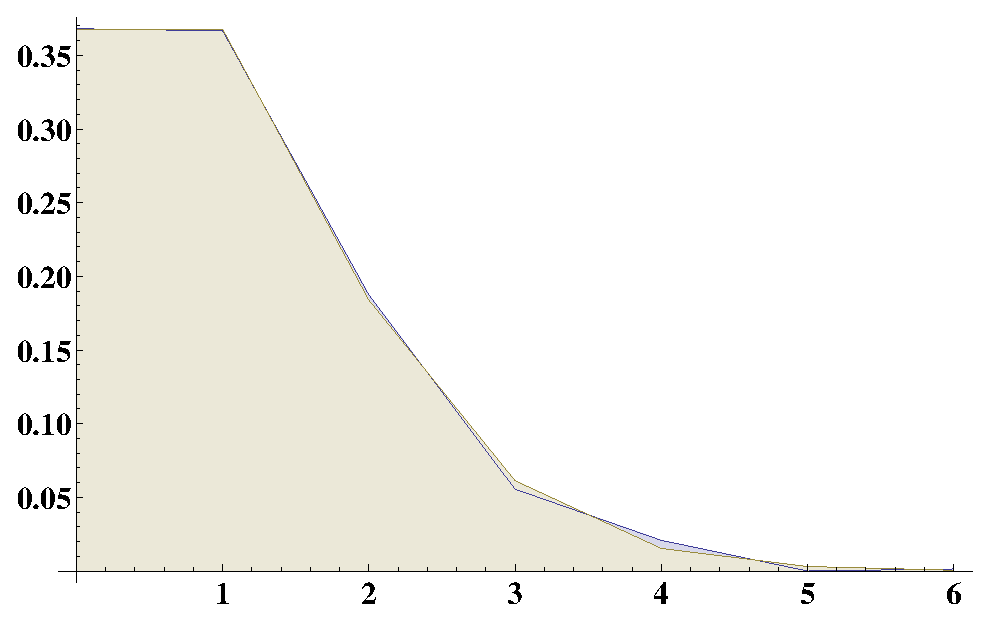
\includegraphics[scale=0.4]{img/n6.eps}
  }
  \caption{Values of $ \Pr{X=k}$ and $ \Pr{Y=k}$\label{fig:diff}}
\end{figure}

We can then conclude that Poisson distribution is a very good approximation to $ X$.
\\

It is worth mentioning that since we have
\[ \dfrac{1}{e}\sum_{k=0}^{\infty}\dfrac{k^n}{k!} = B_n\]
by the famous \emph{Dobinski's formula}\cite{wiki_dob}, therefore $\E{Y^n} = B_n$. This indicates that $ X$ and
$ Y$ also have the same first $ n$ moments.

\subsection{Approximation of $ D_n$}
Inspired by the previous discussion, we now consider the difference between $ D_n $ and $ e^{-1}n!$.

It is obvious that
\begin{align*}
|n! e^{-1} - D_n| & \le \dfrac{1}{(n+1)}+\dfrac{1}{(n+1)(n+2)}+ \dfrac{1}{(n+1)(n+2)(n+3)}+\cdots \\
&< \dfrac{1}{(n+1)} + \dfrac{1}{(n+1)^2 }+ \cdots  \\
& =\dfrac{1}{n}\\
& \le \dfrac{1}{2} ( n \ge 2)
\end{align*}
And for $ n=1,$ we still have $ |n!e^{-1}-D_n| < \dfrac{1}{2}.$

But knowing that $ D_n$ is an integer, we immediately get a neat form of $ D_n$:
\[  D_n = [ n!e^{-1}]\]
where $ [x]$ denote the nearest integer of $ x$, and consequently,
\[ \Pr{X=k} = \dfrac{{n\choose{k}}[(n-k)!e^{-1}]}{n!}= \dfrac{[(n-k)!e^{-1}]}{(n-k)!k!}\]
We then clearly see a beautiful result (which is also shown by \eqnref{def-p}):
\[ \lim\limits_{n\to\infty}\dfrac{D_n}{n!} = \dfrac{1}{e}.\]

